\documentclass[12pt]{article}

\usepackage{wrapfig}
\usepackage{float}
\usepackage{graphicx}
\usepackage[margin=1in]{geometry} 
\usepackage{comment}
\usepackage{amsmath,amsthm,amssymb}
\usepackage{hyperref}
% \usepackage[vlined,linesnumbered,ruled,resetcount]{algorithm2e}

\DeclareMathOperator*{\argmax}{arg\,max}
\DeclareMathOperator*{\argmin}{arg\,min}
\DeclareMathOperator*{\val}{val}
\DeclareMathOperator*{\MOSM}{MOSM}
\DeclareMathOperator*{\WOSM}{WOSM}
\DeclareMathOperator*{\best}{best}
\DeclareMathOperator*{\worst}{worst}

\usepackage{algorithm}
% \usepackage{algorithmicx}
\usepackage[noend]{algpseudocode}

\newcommand{\R}{\mathbb{R}}
\newcommand{\Rgz}{\mathbb{R}_{\ge 0}}
\newcommand{\N}{\mathbb{N}}
\newcommand{\Z}{\mathbb{Z}}

\newcommand{\Es}[2]{\mathbb{E}_{#1}\left[{#2}\right]}
\newcommand{\E}[1]{\mathbb{E}\left[{#1}\right]}
\newcommand{\ip}[2]{\left\langle{#1} , {#2}\right\rangle}

\newcommand{\M}{\mathcal{M}}
\newcommand{\W}{\mathcal{W}}

\newtheorem{definition}{Definition}
\newtheorem{lemma}[definition]{Lemma}
\newtheorem{corollary}[definition]{Corollary}
\newtheorem{theorem}[definition]{Theorem}
\newtheorem{claim}[definition]{Claim}
\newtheorem{proposition}[definition]{Proposition}

\usepackage{filecontents}
\begin{filecontents*}{\jobname.bib}

@article{ThurberConcerningMaxStab02,
  author = {Thurber, Edward G.},
  title = {Concerning the maximum number of stable matchings in the stable
    marriage problem},
  journal = {Discrete Mathematics},
  year = {2002},
  volume = { 248 },
  pages = {195-219},
}
@article{IrvingCountingStab86,
  author    = {Robert W. Irving and
               Paul Leather},
  title     = {The Complexity of Counting Stable Marriages},
  journal   = {{SIAM} J. Comput.},
  volume    = {15},
  number    = {3},
  pages     = {655--667},
  year      = {1986},
  url       = {https://doi.org/10.1137/0215048},
  doi       = {10.1137/0215048},
  timestamp = {Sat, 27 May 2017 14:22:59 +0200},
  biburl    = {https://dblp.org/rec/bib/journals/siamcomp/IrvingL86},
  bibsource = {dblp computer science bibliography, https://dblp.org}
}
@article{PittelAverageStable89,
  author = {Pittel, B.},
  title = {The Average Number of Stable Matchings},
  journal = {SIAM J. Discret. Math.},
  issue_date = {Nov. 1989},
  volume = {2},
  number = {4},
  month = nov,
  year = {1989},
  issn = {0895-4801},
  pages = {530--549},
  numpages = {20},
  url = {http://dx.doi.org/10.1137/0402048},
  doi = {10.1137/0402048},
  acmid = {75544},
  publisher = {Society for Industrial and Applied Mathematics},
  address = {Philadelphia, PA, USA},
}
@misc {ShorAsymptoticStab19,
  TITLE = {The asymptotic behavior of a recurrence related to stable matchings},
  AUTHOR = {Peter Shor },
  HOWPUBLISHED = {Theoretical Computer Science Stack Exchange},
  NOTE = {URL: \url{https://cstheory.stackexchange.com/q/44371} (version: 2019-08-08)},
  EPRINT = {https://cstheory.stackexchange.com/q/44371},
  URL = {https://cstheory.stackexchange.com/q/44371}
}
\end{filecontents*}

\begin{document}

% \renewcommand{\qedsymbol}{\filledbox}
 
\title{
  A recurrence giving a lower bound for stable matchings
}
\author{Clay Thomas\\
claytont@princeton.edu}
\maketitle

It's an interesting open question to find good upper and lower bounds on the
maximum number of distinct stable matches that an $n\times n$ instance of the
stable marriages problem can have.
The best known lower bound (for $n$ a power of $2$) was originally constructed
in \cite{IrvingCountingStab86},
and a recurrence relation for the lower bound was found.
Specifically, define
  \[ b_0 = 1, \qquad b_1 = 2 \]
  \[ b_n = 3 b_{n-1}^2 - 2 b_{n-2}^4, \qquad n > 1 \]
Then $b_n$ gives a lower bound on the maximum number of stable matches in
a $2^n \times 2^n$ instance.
For a justification of this recurrence, see \cite{ThurberConcerningMaxStab02},
appendix A.
Knuth analyzed $b_n$ and found it was $\Omega(2.28^{2^n})$
(mentioned, e.g. in \cite{PittelAverageStable89}).
However, the details of this analysis were, to the best of our knowledge,
never published.
In this note, we establish the growth behavior of the sequence,
following the proof given by Peter Shor \cite{ShorAsymptoticStab19}.

\begin{proposition}
  There exist constants $s, r$ such that $b_n \sim r s^{2^n}$,
  i.e. $b_n = rs^{2^n}(1 + o(1))$.
  Moreover, $s\approx 2.280142$ and $r = \frac 1 2 (\sqrt 3 - 1) 
  \approx 0.366025$
\end{proposition}

First, note that this is plausible because, if $c_n = 3 c_{n-1}^2$ (i.e. if we
eliminated the lower order terms of the recurrence)
we would have $c_n = (1/3) s^{2^n}$ where $s=3c_0$.
Now, if we had $b_n = r s^{2^n}$ exactly, we could recover $r$ and $s$ as
follows: $r = b_{n-1}^2 / b_n$ and
$s = \left(\frac{b_n}{r}\right)^{1/2^n}$ for any value of $n$.
In fact, we'll show that the above quantities \emph{quickly converge} to some
values $r$ and $s$ which produce the desired result.

\begin{proof}
First we handle $r$. Define
\[ r_n = \frac{b_{n-1}^2}{b_n} \]

\begin{claim}
  $r_n \to r$ as $n\to \infty$ for some value $r$.
  Moreover, $r_n$ monotonically decreases to $r$.
\end{claim}
\begin{proof}
  Because $r_n \ge 0$, it suffices to show that $r_n$ is decreasing.
  We have
  \[ r_n = \frac{b_{n-1}^2}{b_n}
  = \frac{b_{n-1}^2}{3b_{n-1}^2 - 2b_{n-2}^4}
  = \frac{1}{3 - 2(b_{n-2}^2/b_{n-1})^2}
  = \frac{1}{ 3 - 2r_{n-1}^2} \]
  Now, $r_1 = 1/2$, and we can easily see from a graph that the function
  $f(x) = 1/(3-2x^2)$ that $f(x) \le x$ for $r < x < 1$, where
  $r \approx 0.366$. (In particular, $r = (\sqrt 3 - 1)/2$ is the smaller
  positive root of $x(3-2x^2)=1$).
  Moreover, for $r < x < 1$ we have $f(x) > r$ as well.
  Thus, $r_n < r_{n-1}$ for all $n > 0$.

\end{proof}

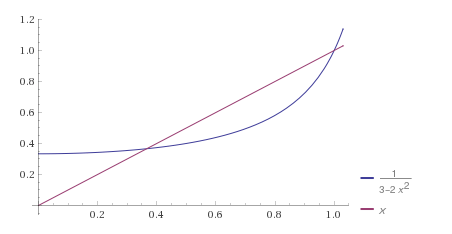
\includegraphics{RatioConvergencePlot}

Note that certainly $r > 0$.
Now we can turn to $s$. Define
\[ s_n = \left(\frac{b_n}{r}\right)^{1/2^n} \]

\begin{claim}
  $s_n \to s$ as $n\to \infty$ for some value $s$.
  Moreover, $s_n$ monotonically decreases to $s$.
\end{claim}
\begin{proof}
  Because $s_n \ge 0$, it suffices to show that
  $s_n$ is decreasing.
  We have
  \[ \frac{s_{n}}{s_{n-1}}
    = \left(\frac{b_n}{r}\right)^{1/2^n} \left(\frac{r}{b_{n-1}}\right)^{2/2^n}
    = \left(\frac{rb_n}{b_{n-1}^2}\right)^{1/2^n}
    = \left(\frac{r}{r_n}\right)^{1/2^n} < 1
  \]
  where the inequality follows because $r_n > r$.
  Thus $s_n < s_{n-1}$, as desired.
\end{proof}

So far, we have $b_n = r s_n^{2^n} \ge r s^{2^n}$.
All that remains is to show that, in fact,
$b_n \le rs^{2^n}(1 + o(1))$ as well.

\begin{claim}
  $s^{2^n} / s_n^{2^n} \to 1$ as $n\to \infty$
\end{claim}
\begin{proof}
  As $s_n \ge s$, we know $(s/s_n)^{2^n} \le 1$.
  We have
  \[ \left(\frac{s}{s_n}\right)^{2^n}
  = \left(\prod_{k=n}^\infty \frac{s_{k+1}}{s_k}\right)^{2^n}
  = \prod_{k=n}^\infty \left(\frac{r}{r_{k+1}}\right)^{\frac{1}{2^{k+1}}\cdot 2^n}
  \]
  \[ \ge \prod_{k=n}^\infty \left(\frac{r}{r_{n+1}}\right)^{\frac{1}{2^{k+1}}\cdot 2^n}
  = \left(\frac{r}{r_{n+1}}\right)^{ 2^n\cdot\sum_{k=n}^\infty \frac{1}{2^{k+1}}\cdot}
  = \frac{r}{r_{n+1}}
  \]
  The inequality follows from the fact that $r_n$ is decreasing.
  The right hand side approaches $1$ by the definition of $r$.
\end{proof}

Thus, we can conclude that 
\[ \frac{b_n}{rs^{2^n}} = \frac{s_n^{2^n}}{s^{2^n}} \to 1 \]
as $n\to \infty$, as desired.
\end{proof}

\paragraph{Remark:}
We saw that $r = (\sqrt 3 - 1)/2$ can be calculated exactly.
Combining a few facts above we can also get highly accurate estimates for $s$.
Specifically, in claims 2, 3, and 4 respectively we showed
\[ r_n = \frac 1 {3 - 2r_{n-1}^2} \]
\[ s_n = s_{n-1} \left(\frac r {r_n}\right)^{1/2^n} \]
\[ s_n \ge s \ge s_n \left(\frac r {r_n}\right)^{1/2^n} \]
The first two lines give us fast ways to compute the estimates of $s_n$, and
the last line shows that this estimate converges extremely quickly
(indeed, all we need to do is observe that $r/r_n$ is bounded by a constant $c$
and that $c^{1/2^n} = 1 - O(1/2^n)$ to get exponential convergence).

\bibliography{\jobname}{}
\bibliographystyle{alpha}

\end{document}

